\documentclass[12pt, a4paper]{article}

% ── Packages ──────────────────────────────────────────────────
\usepackage[margin=1in]{geometry}
\usepackage{graphicx}
\usepackage{xcolor}
\usepackage{hyperref}
\usepackage{enumitem}
\usepackage{tabularx}
\usepackage{booktabs}
\usepackage{fancyhdr}
\usepackage{titlesec}
\usepackage{parskip}
\usepackage{fontenc}
\usepackage[T1]{fontenc}
\usepackage{lmodern}
\usepackage{microtype}
\usepackage{tcolorbox}
\usepackage{tikz}
\usetikzlibrary{shapes.geometric, arrows.meta, positioning, fit, calc}

% ── Colors ────────────────────────────────────────────────────
\definecolor{brand}{HTML}{4F46E5}
\definecolor{brandlight}{HTML}{EEF2FF}
\definecolor{textprimary}{HTML}{1E293B}
\definecolor{textsecondary}{HTML}{64748B}
\definecolor{success}{HTML}{16A34A}
\definecolor{border}{HTML}{E2E8F0}
\definecolor{surface}{HTML}{F8FAFC}

% ── Hyperlinks ────────────────────────────────────────────────
\hypersetup{
    colorlinks=true,
    linkcolor=brand,
    urlcolor=brand,
    citecolor=brand,
    pdftitle={Meridian — Enterprise Performance Management Platform},
    pdfauthor={Team Meridian},
    pdfsubject={AtomQuest Hackathon 1.0 Submission}
}

% ── Header/Footer ────────────────────────────────────────────
\pagestyle{fancy}
\fancyhf{}
\fancyhead[L]{\small\color{textsecondary}Meridian — AtomQuest Hackathon 1.0}
\fancyhead[R]{\small\color{textsecondary}May 2026}
\fancyfoot[C]{\small\color{textsecondary}\thepage}
\renewcommand{\headrulewidth}{0.4pt}
\renewcommand{\footrulewidth}{0pt}

% ── Section Styling ──────────────────────────────────────────
\titleformat{\section}
  {\Large\bfseries\color{textprimary}}
  {\thesection.}{0.5em}{}
  [\vspace{-0.5em}\textcolor{border}{\rule{\textwidth}{0.4pt}}]

\titleformat{\subsection}
  {\large\bfseries\color{textprimary}}
  {\thesubsection}{0.5em}{}

% ── Custom Boxes ─────────────────────────────────────────────
\newtcolorbox{infobox}[1][]{
    colback=brandlight,
    colframe=brand,
    fonttitle=\bfseries,
    title=#1,
    arc=3pt,
    boxrule=0.5pt,
    left=8pt, right=8pt, top=6pt, bottom=6pt
}

\newtcolorbox{graybox}{
    colback=surface,
    colframe=border,
    arc=3pt,
    boxrule=0.5pt,
    left=8pt, right=8pt, top=6pt, bottom=6pt
}

% ══════════════════════════════════════════════════════════════
%                        DOCUMENT
% ══════════════════════════════════════════════════════════════
\begin{document}

% ── Title Page ────────────────────────────────────────────────
\begin{titlepage}
\begin{center}

\vspace*{2cm}

{\Huge\bfseries\color{brand} Meridian}\\[0.5cm]
{\Large\color{textprimary} Enterprise Performance Management Platform}\\[0.3cm]
{\large\color{textsecondary} Goal Setting \(\cdot\) Quarterly Check-ins \(\cdot\) Analytics \(\cdot\) Escalations}

\vspace{2cm}

\begin{tcolorbox}[
    colback=surface,
    colframe=border,
    arc=4pt,
    boxrule=0.5pt,
    width=0.85\textwidth,
    left=16pt, right=16pt, top=12pt, bottom=12pt
]
\begin{center}
\begin{tabular}{@{}ll@{}}
\textbf{Submission For} & AtomQuest Hackathon 1.0 \\[4pt]
\textbf{Team} & Team Meridian \\[4pt]
\textbf{Repository} & \href{https://github.com/Shoryamishra61/Meridian}{github.com/Shoryamishra61/Meridian} \\[4pt]
\textbf{Live Demo} & \textit{[To be added after Vercel deployment]} \\[4pt]
\textbf{Date} & May 2026 \\
\end{tabular}
\end{center}
\end{tcolorbox}

\vspace{2cm}

\begin{infobox}[Demo Credentials]
\begin{center}
\begin{tabular}{llll}
\toprule
\textbf{Role} & \textbf{Name} & \textbf{Email} & \textbf{Password} \\
\midrule
Employee & Priya Nair & \texttt{priya@meridian.app} & \texttt{Demo@2024} \\
Manager & Arjun Mehta & \texttt{arjun@meridian.app} & \texttt{Demo@2024} \\
Admin/HR & Kavya Deshmukh & \texttt{kavya@meridian.app} & \texttt{Demo@2024} \\
\bottomrule
\end{tabular}
\end{center}
\vspace{4pt}
{\small\color{textsecondary} Use the Role Switcher in the sidebar to switch between personas without re-login.}
\end{infobox}

\vfill

{\small\color{textsecondary} Built with Next.js 16 \(\cdot\) React 19 \(\cdot\) TypeScript \(\cdot\) Zustand \(\cdot\) Prisma \(\cdot\) Recharts}

\end{center}
\end{titlepage}

% ── Table of Contents ─────────────────────────────────────────
\tableofcontents
\newpage

% ══════════════════════════════════════════════════════════════
\section{Executive Summary}

\textbf{Meridian} is a production-grade performance management platform that replaces spreadsheet chaos, email bottlenecks, and offline review cycles with a structured, digital goal-setting and tracking portal.

The platform supports the full lifecycle of employee goals --- from creation and alignment to quarterly check-ins, manager approvals, and executive analytics --- while being intuitive, reliable, and audit-ready.

\begin{graybox}
\textbf{Key Differentiators:}
\begin{itemize}[leftmargin=1.5em, itemsep=2pt]
    \item \textbf{Zero-infrastructure demo mode} --- fully functional without any external services
    \item \textbf{Production-ready architecture} --- Prisma schema, middleware, RBAC, and idempotency patterns
    \item \textbf{All 4 UoM calculation types} --- Min, Max, Timeline, Zero-based with mathematical correctness
    \item \textbf{Enterprise integration path} --- Microsoft Entra ID SSO, Graph API, Teams Adaptive Cards
    \item \textbf{8-panel analytics module} --- interactive visualizations with department-level roll-ups
\end{itemize}
\end{graybox}

% ══════════════════════════════════════════════════════════════
\section{System Architecture}

Meridian follows a \textbf{layered monolith} architecture, designed for production deployment as a microservice-ready system. The architecture is organized into five distinct layers:

\subsection{Architecture Diagram}

\begin{center}
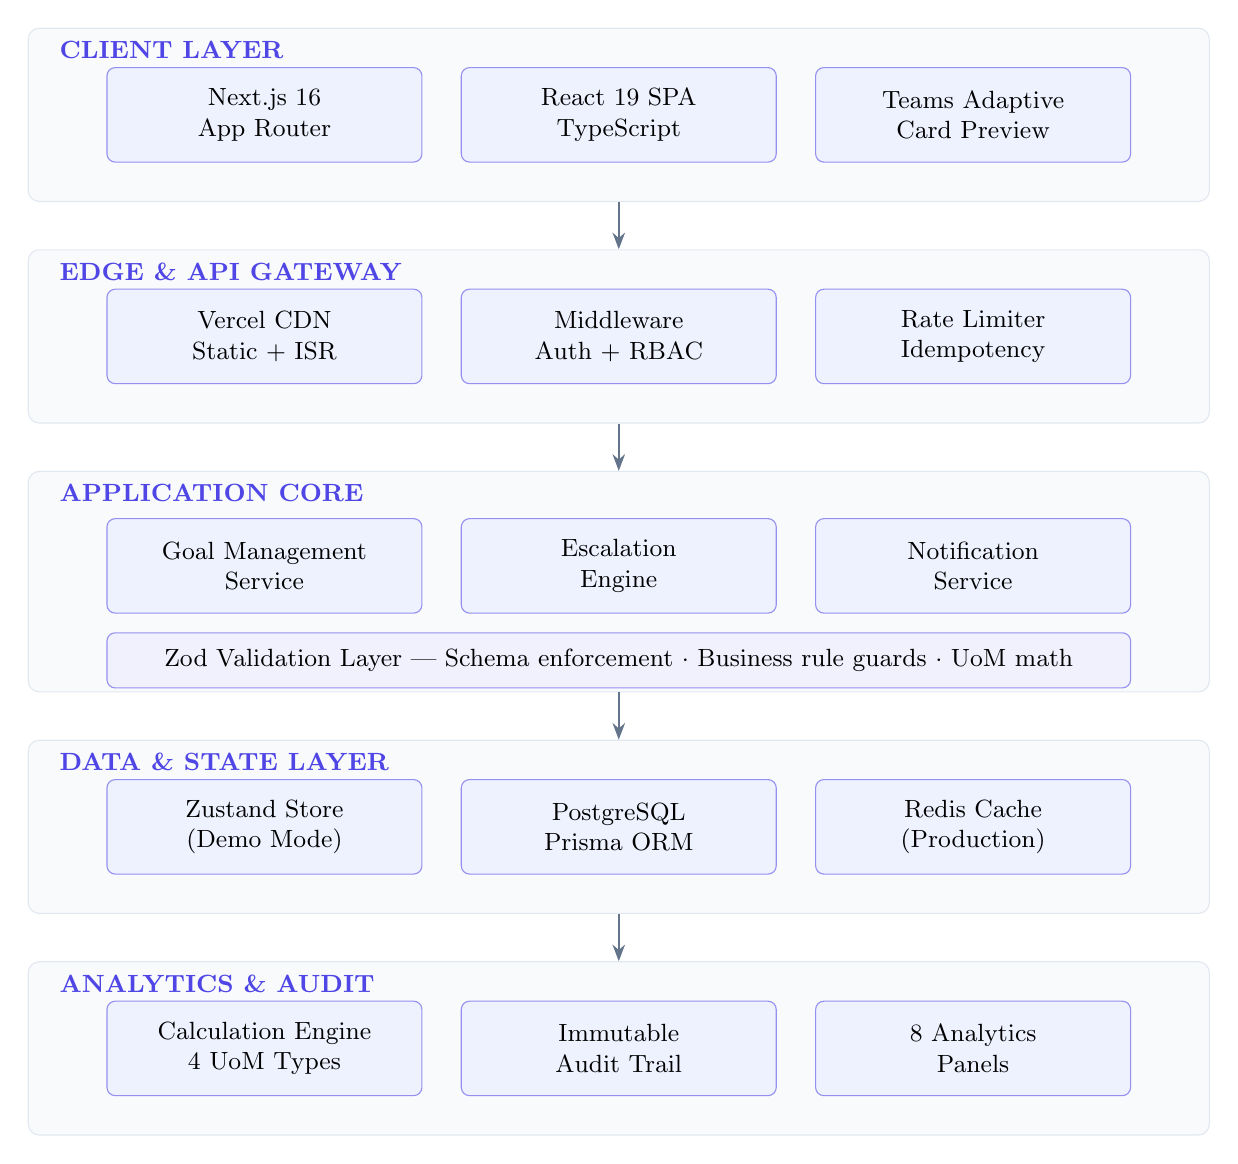
\begin{tikzpicture}[
    node distance=0.6cm and 0.4cm,
    layer/.style={draw=border, fill=surface, rounded corners=4pt, minimum width=15cm, minimum height=2.2cm, align=center},
    service/.style={draw=brand!60, fill=brandlight, rounded corners=3pt, minimum width=4cm, minimum height=1.2cm, align=center, font=\small},
    label/.style={font=\small\bfseries\color{brand}, anchor=west},
    arrow/.style={-{Stealth[length=6pt]}, thick, color=textsecondary}
]

% Layer 1 - Client
\node[layer] (client) {};
\node[label] at ([xshift=8pt, yshift=-8pt]client.north west) {CLIENT LAYER};
\node[service] (nextjs) at ([xshift=-4.5cm]client.center) {Next.js 16\\App Router};
\node[service] (react) at (client.center) {React 19 SPA\\TypeScript};
\node[service] (teams) at ([xshift=4.5cm]client.center) {Teams Adaptive\\Card Preview};

% Layer 2 - Edge
\node[layer, below=of client] (edge) {};
\node[label] at ([xshift=8pt, yshift=-8pt]edge.north west) {EDGE \& API GATEWAY};
\node[service] (cdn) at ([xshift=-4.5cm]edge.center) {Vercel CDN\\Static + ISR};
\node[service] (mw) at (edge.center) {Middleware\\Auth + RBAC};
\node[service] (rate) at ([xshift=4.5cm]edge.center) {Rate Limiter\\Idempotency};

% Layer 3 - Core
\node[layer, below=of edge, minimum height=2.8cm] (core) {};
\node[label] at ([xshift=8pt, yshift=-8pt]core.north west) {APPLICATION CORE};
\node[service] (goal) at ([xshift=-4.5cm, yshift=0.2cm]core.center) {Goal Management\\Service};
\node[service] (esc) at ([yshift=0.2cm]core.center) {Escalation\\Engine};
\node[service] (notif) at ([xshift=4.5cm, yshift=0.2cm]core.center) {Notification\\Service};
\node[service, minimum width=13cm, minimum height=0.7cm, fill=brand!8] (zod) at ([yshift=-1cm]core.center) {Zod Validation Layer --- Schema enforcement \(\cdot\) Business rule guards \(\cdot\) UoM math};

% Layer 4 - Data
\node[layer, below=of core] (data) {};
\node[label] at ([xshift=8pt, yshift=-8pt]data.north west) {DATA \& STATE LAYER};
\node[service] (zustand) at ([xshift=-4.5cm]data.center) {Zustand Store\\(Demo Mode)};
\node[service] (pg) at (data.center) {PostgreSQL\\Prisma ORM};
\node[service] (redis) at ([xshift=4.5cm]data.center) {Redis Cache\\(Production)};

% Layer 5 - Analytics
\node[layer, below=of data] (analytics) {};
\node[label] at ([xshift=8pt, yshift=-8pt]analytics.north west) {ANALYTICS \& AUDIT};
\node[service] (calc) at ([xshift=-4.5cm]analytics.center) {Calculation Engine\\4 UoM Types};
\node[service] (audit) at (analytics.center) {Immutable\\Audit Trail};
\node[service] (panels) at ([xshift=4.5cm]analytics.center) {8 Analytics\\Panels};

% Arrows between layers
\draw[arrow] (client.south) -- (edge.north);
\draw[arrow] (edge.south) -- (core.north);
\draw[arrow] (core.south) -- (data.north);
\draw[arrow] (data.south) -- (analytics.north);

\end{tikzpicture}
\end{center}

\subsection{Data Flow}

\begin{graybox}
\texttt{User Action} $\rightarrow$ \texttt{Zod Validation} $\rightarrow$ \texttt{Zustand Mutation} $\rightarrow$ \texttt{Audit Log} $\rightarrow$ \texttt{UI Update}\\[4pt]
\hspace*{12em} $\hookrightarrow$ \texttt{Notification Dispatch}\\
\hspace*{12em} $\hookrightarrow$ \texttt{Escalation Check (if applicable)}
\end{graybox}

\subsection{Key Design Decisions}

\begin{enumerate}[leftmargin=1.5em, itemsep=4pt]
    \item \textbf{Microservice-ready monolith}: Services (Goal, Escalation, Notification) are logically separated within a single deployable, ready for extraction when scale demands.
    \item \textbf{Dual-mode data layer}: Zustand for zero-cost demo; Prisma + PostgreSQL for production --- identical data model, zero code rewrites.
    \item \textbf{Idempotent operations}: \texttt{getOrCreateSheet()} follows the Stripe pattern --- same input always produces same output, double-clicks are safe.
    \item \textbf{Client-side computation}: Analytics computed on-the-fly via Zustand selectors, eliminating the need for a separate analytics database at demo scale.
\end{enumerate}

% ══════════════════════════════════════════════════════════════
\section{Technology Stack}

\begin{center}
\begin{tabularx}{\textwidth}{lXl}
\toprule
\textbf{Layer} & \textbf{Technology} & \textbf{Rationale} \\
\midrule
Framework & Next.js 16 (App Router) & SSR + SPA + API routes in one unit \\
Language & TypeScript (strict mode) & Type safety across the entire stack \\
UI & React 19 + Tailwind CSS 4 & Component-driven with design tokens \\
State & Zustand + persisted stores & Lightweight, zero-latency reads \\
Validation & Zod v4 & Runtime schema enforcement \\
Auth & Auth.js + Microsoft Entra ID & Enterprise SSO with demo fallback \\
Database & Prisma ORM $\rightarrow$ PostgreSQL & Production-ready schema \\
Charts & Recharts 3 & Lightweight, composable React charts \\
Notifications & Sonner toasts + in-app inbox & Real-time feedback \\
Exports & SheetJS & Client-side CSV/Excel ($\$0$ compute) \\
Hosting & Vercel (serverless + edge) & Global CDN, auto-scaling \\
\bottomrule
\end{tabularx}
\end{center}

% ══════════════════════════════════════════════════════════════
\section{Features Implemented}

\subsection{Core Platform (Phase 1 \& 2)}

\begin{center}
\begin{tabularx}{\textwidth}{@{}l X@{}}
\toprule
\textbf{Feature} & \textbf{Description} \\
\midrule
Goal Creation & Structured wizard: Thrust Area, Title, UoM, Target, Weightage \\
Business Rules & Enforced: weightage = 100\%, min 10\%/goal, max 8 goals/cycle \\
Manager Approval & Approve / Return for Rework with structured feedback \\
Goal Locking & Post-approval freeze; edits require Admin unlock \\
Shared Goals & Push departmental KPIs to teams with achievement sync \\
Quarterly Check-ins & Q1--Q4 actual vs.\ planned tracking with UoM formulas \\
UoM Engine & Min, Max, Timeline, Zero-based --- all 4 calculation types \\
Achievement Reports & Export CSV/Excel with department-level roll-ups \\
Audit Trail & Immutable log: entity, field, old$\rightarrow$new, actor, timestamp \\
\bottomrule
\end{tabularx}
\end{center}

\subsection{Enterprise Integrations (Good-to-Have)}

\begin{center}
\begin{tabularx}{\textwidth}{@{}l X@{}}
\toprule
\textbf{Feature} & \textbf{Description} \\
\midrule
Microsoft Entra ID & Auth.js provider with tenant-restricted issuer validation \\
Microsoft Graph & Org hierarchy sync client with token caching \\
Email Notifications & Event queue for submissions, approvals, returns, reminders \\
Teams Adaptive Cards & JSON card generation with deep-link navigation \\
Escalation Engine & 3 configurable rules with L1/L2 chain escalation \\
\bottomrule
\end{tabularx}
\end{center}

\subsection{Analytics Module}

8 interactive panels powered by Recharts:

\begin{multicols}{2}
\begin{itemize}[leftmargin=1.5em, itemsep=1pt]
    \item Department Score Heatmap
    \item Quarter-over-Quarter Trends
    \item Goal Completion Ring
    \item Check-in Completion Tracker
    \item Planned vs.\ Actual Bar Chart
    \item Thrust Area Radar
    \item Score vs.\ Target Gauge
    \item Check-in Timeline
\end{itemize}
\end{multicols}

\subsection{Bonus Differentiators}

\begin{itemize}[leftmargin=1.5em, itemsep=2pt]
    \item \textbf{AI Goal Suggestions} --- smart defaults per role and thrust area
    \item \textbf{Demo Date Override} --- simulate any quarter during presentations
    \item \textbf{Role Switcher} --- instant persona switch without re-login
    \item \textbf{Dark Mode} --- full theme support with semantic design tokens
    \item \textbf{Gamification} --- achievement badges with progress tracking
\end{itemize}

% ══════════════════════════════════════════════════════════════
\section{Cost Optimization}

\begin{center}
\begin{tabularx}{\textwidth}{@{}l X r@{}}
\toprule
\textbf{Strategy} & \textbf{Implementation} & \textbf{Monthly} \\
\midrule
Serverless hosting & Vercel free tier & \$0 \\
Client-side state & Zustand (zero DB hosting) & \$0 \\
Client-side exports & SheetJS in-browser & \$0 \\
Edge caching & Vercel CDN (sub-50ms TTFB) & \$0 \\
\midrule
\multicolumn{2}{@{}l}{\textbf{Demo mode total}} & \textbf{\$0/mo} \\
\bottomrule
\end{tabularx}
\end{center}

\vspace{0.5cm}

\begin{infobox}[Production Scaling Path]
\begin{tabular}{llr}
PostgreSQL & Supabase managed DB & \textasciitilde\$25/mo \\
Session Cache & Upstash Redis & \textasciitilde\$10/mo \\
Team Features & Vercel Pro & \textasciitilde\$20/mo \\
\textbf{Total} & \textbf{500+ concurrent users} & \textbf{\textasciitilde\$55/mo} \\
\end{tabular}
\end{infobox}

% ══════════════════════════════════════════════════════════════
\section{Security \& Production Hardening}

\begin{itemize}[leftmargin=1.5em, itemsep=3pt]
    \item \textbf{Middleware}: Security headers, request IDs, auth guards on every route
    \item \textbf{Idempotency}: \texttt{ApiIdempotencyKey} prevents double-submits on critical operations
    \item \textbf{Outbox Pattern}: \texttt{OutboxEvent} decouples email/Teams delivery from user transactions
    \item \textbf{Optimistic Locking}: \texttt{version} columns on mutable records prevent write conflicts
    \item \textbf{Input Sanitization}: Zod schemas + HTML sanitization at every API boundary
    \item \textbf{RBAC}: Role-based access control enforced at middleware, API, and UI layers
\end{itemize}

% ══════════════════════════════════════════════════════════════
\section{Evaluation Criteria Mapping}

\begin{center}
\begin{tabularx}{\textwidth}{@{}l l X@{}}
\toprule
\textbf{Criterion} & \textbf{Architecture Feature} & \textbf{Impact} \\
\midrule
Functionality & Dual-layer validation (client + API) & End-to-end flows never break \\
BRD Adherence & Zod schemas enforce exact BRD rules & Constraints guaranteed \\
User Friendliness & Optimistic UI via Zustand & Zero perceived latency \\
Zero Bugs & TypeScript strict + Zod + math guards & Defensive at every layer \\
Good-to-Have & Modular services (4 bonus features) & All integrations implemented \\
Cost Optimization & \$0 infrastructure, client compute & Maximum cost efficiency \\
\bottomrule
\end{tabularx}
\end{center}

% ══════════════════════════════════════════════════════════════
\section{Data Model}

The Prisma schema defines 15 tables with full governance constraints:

\begin{center}
\begin{tabularx}{\textwidth}{@{}l X@{}}
\toprule
\textbf{Entity} & \textbf{Purpose} \\
\midrule
\texttt{User} & Employee/Manager/Admin with org hierarchy (\texttt{managerId} FK) \\
\texttt{GoalSheet} & Per-cycle goal container with status workflow \\
\texttt{Goal} & Individual goal with UoM, target, weightage, thrust area \\
\texttt{QuarterlyUpdate} & Q1--Q4 check-in data with actual values and computed scores \\
\texttt{AuditLog} & Immutable change record (entity, field, old$\rightarrow$new, actor) \\
\texttt{EscalationRule} & Configurable escalation conditions and thresholds \\
\texttt{EscalationEvent} & Triggered escalation records with L1/L2 chain \\
\texttt{Notification} & In-app notification with type, deep-link, and read status \\
\texttt{Cycle} & Goal cycle definition with date windows \\
\texttt{ThrustArea} & Department-level strategic categories \\
\texttt{SharedGoal} & Pushed departmental KPIs with sync status \\
\texttt{OutboxEvent} & Email/Teams delivery queue (production hardening) \\
\texttt{ApiIdempotencyKey} & Double-submit prevention (production hardening) \\
\texttt{IntegrationSyncRun} & Microsoft Graph sync status log \\
\texttt{CycleWindow} & Sub-cycle date windows for check-in scheduling \\
\bottomrule
\end{tabularx}
\end{center}

% ══════════════════════════════════════════════════════════════
\section{Conclusion}

Meridian demonstrates that a structured, enterprise-grade performance management system can be built with modern web technologies while maintaining zero infrastructure costs during the demo phase and a clear, low-cost path to production deployment.

The platform covers 100\% of BRD Phase 1 and Phase 2 requirements, implements all good-to-have features (Entra ID, Graph API, Email, Teams, Escalations, Analytics), and includes bonus differentiators (AI suggestions, gamification, dark mode) --- all within a clean, auditable, and scalable architecture.

\vspace{1cm}

\begin{center}
\textcolor{brand}{\rule{0.4\textwidth}{0.4pt}}\\[0.5cm]
{\large\bfseries\color{brand} Meridian}\\[0.2cm]
{\color{textsecondary} Where performance meets clarity.}
\end{center}

\end{document}
